 
\documentclass[a4paper,12pt]{diplom}
% \usepackage[latin1]{inputenc}
% \usepackage[utf8]{inputenc}
\inputencoding{utf8} % Кодировка вашего файла


\usepackage{paratype} % Шрифты (можно отключить, если дает ошибку)
%% Немного увеличим шрифт в математическом режиме, чтобы соответствовать размерам Paratype-шрифтов
\DeclareMathSizes{12}{13.4}{11}{10}

\usepackage[left=3cm,right=2cm,top=2cm,bottom=2cm]{geometry} % Размеры полей
\usepackage[onehalfspacing]{setspace} % Полуторный интервал
%\renewcommand{\baselinestretch}{1.25} % Полуторный интервал
\usepackage{indentfirst} % Абзацный отступ в начале разделов
\setlength{\parindent}{1.25cm} % Величина абзацного отступа

\usepackage[pdftex]{graphicx} % Для вставки изображений
\usepackage{array} % Для таблиц
\usepackage{booktabs} % Для красивых таблиц 
\usepackage{tikz} % Рисунки с помощью TikZ
\usepackage[linesnumbered,lined,ruled]{algorithm2e} % Для оформления псевдокода
%\usepackage{algorithm} % Альтернатива оформления псевдокода
%\usepackage{algpseudocode} % Альтернатива оформления псевдокода
\usepackage{listings} % Оформление листингов программ
\usepackage{icomma} % Удаляем тонкий пробел после запятой в мат. режиме

% Если на нумерованную формулу нет ссылки в тексте,
\mathtoolsset{showonlyrefs} % то она становится ненумерованной

% microtype улучшает распределение символов в строке
\usepackage{microtype}  % Можно отключить, если возникают ошибки компиляции

% Формируем PDF с полноценными перекрестными ссылками
\usepackage[unicode, pdfborder={0 0 0}, pdfstartview=FitV]{hyperref}

% Часто используемые макросы
\newcommand{\N}{\mathbb{N}}  % Множество натуральных чисел
\newcommand{\Z}{\mathbb{Z}}  % Множество целых чисел
\newcommand{\R}{\mathbb{R}}  % Множество действительных чисел
\DeclareMathOperator{\sgn}{sgn} % Знак числа
\DeclareMathOperator{\M}{\mathsf{M}} % Матожидание
\newcommand{\from}{\colon} % Двоеточие в определении функции. Пример: $f \from \R \to \N$.
% Заменяем англоязычные обозначения на русские
\renewcommand{\le}{\leqslant}
\renewcommand{\leq}{\leqslant}
\renewcommand{\ge}{\geqslant}
\renewcommand{\geq}{\geqslant}
\renewcommand{\emptyset}{\varnothing}
\renewcommand{\epsilon}{\varepsilon}


%%%%%%%%%%%%%%%%%%%%%%%%%%
% Конец преамбулы
%%%%%%%%%%%%%%%%%%%%%%%%%%

% ==================== Титульный лист ====================

\begin{document}

% Содержимое титульного листа

%\LetterHead{Минобр...}
\Kafedra{Кафедра информатики}

% Зав. кафедрой
\ZavKaf{Заведующий кафедрой,\\ д.\,ф.-м.\,н., профессор}{С.\,С.~Сидоров}
% Если это курсовая работа и виза зав. каф. не нужна, раскомментируйте следующую строку
%\Kursovaya

% Вид работы: Курсовая работа, Выпускная квалификационная работа, 
\DocumentType{\large Выпускная квалификационная работа}

% Название дипломной работы
\Title{\begin{Large}\bfseries Методы обратной свертки в задачах \\ космической физики\end{Large}}

% Направление подготовки
\Napr{по направлению\\ 02.03.02 Прикладная математика и информатика}

% Руководитель
\Chief{Научный руководитель\\ к.\,ф.-м.\,н., доцент}{Ю.\,В.~Богомолов}

% Автор
\Author{Студент группы ИВТ-21МО}{А.\,В.~Ющенко}

%\City{Ярославль}
%\Year{2017}





\maketitle
\chapter{Реферат}

Объем \total{page} с., \total{chapternum} гл., \total{fignum} рис.,
\total{tablenum} табл., \total{bibnum} источников, \total{appnum} прил.

\medskip

Ключевые слова: \textbf{Обратная свертка, Unfolding, SVD}

\medskip

На сегодняшний день электронные измерительные приборы используются повсеместно, почти не осталось отраслей для применения аналоговых приборов. 
Однако результаты измерений могут быть искажены и трансформированы, из-за множества факторов. Одной из областей нуждающихся в поиске истинных 
значений является космическая физика. Так же усложнением задачи являться то, что нужно восстанавливать многомерные измеренные спектры 
космических частиц. Для решения данной задачи в работе предлагается рассмотреть SVD (Singular Value Decomposition) подход для решения задачи 
обратной свертки, которая возникает при построении матрицы миграций. А именно будут расстроены: подход к решению многомерной задачи через 
решение $n$ одномерных, и подход с нелинейным отношением соседства.


\tableofcontents[Содержание]


\chapternonum{Введение}

В космической физике измерения наблюдаемых — спектров инвариантных массы, угловые распределения частиц и прочее — обычно искажаются 
и трансформируются различными эффектами, такими как конечное разрешение аппаратуры или ограниченный приемник детектора. По этой причине 
часто невозможно или, по крайней мере, очень трудно провести прямое сравнение данных, полученных с помощью разных детекторов, друг с другом 
и с различными теоретическими прогнозами. Например исходный спектр может быть сжат или сдвинут, либо вообще изменен не линейным преобразованием. 
Чтобы преодолеть эту проблему, некоторые исследования чрезмерно заботятся о процессе измерения. В идеале в результате этих исследований должна 
получиться функция с двумя переменными, описывающая отклик детектора, чтобы фактическое измеренное распределение можно было рассматривать как 
свертку этой функции с истинным. В общем случае это приводит к интегральному уравнению для истинного распределения. Решение этого уравнения 
(т.е. \textit{развертывание} истинного распределения) обычно требует некоторой дискретизации, что приводит к системе линейных уравнений. 
Однако задача относится к классу некорректных задач, неустойчивых к малым изменениям исходной системы. Из-за неизбежных статистических 
ошибок в измеренном распределении точное решение (если оно существует) обычно сильно колеблется и в конечном итоге бесполезно. 

Еще одним подходом может для решения этой задачи может быть задача анфолдинга ( от англ. Unfolding ) или обратной свертки. Зная о дефектах 
приборов можно создать математическую модель, с помощью которой построить качественные оценки распределений, и использовать их для решения 
задачи обратной свертки. При таком подходе необходимо разбить множество допустимых значений на интервалы и посчитать гистограмму 
( количество попаданий в каждый интервал ), далее следуют определить вероятности попадания истинного распределения в i бин ( интервал ) 
при условии что измеренная частица попала в j бин. На основе этих данных строится матрица миграций и уже сверка измеренного спектра с ней, 
даст оценку истинного распределения.

Одним из способов решения задачи анфолдинга, может быть SVD ( Singulav Value Decomposition ) алгоритм. Главным его достоинством является
возможность учитывать характер исходного распределения, например, непрерывность или гладкость. Данный подход называется регулязационным
и широко применяется для решения одномерной задачи.

При работе с космическими частицами, физическая величина может оказаться многомерной, в данный работе  рассмотренные частицы со следующими
характеристиками: направление, жесткость и энергия. Для подобных задач стандартный методом регулязации не подходит, т.к. он может учитывать
только гладкость соседних бинов, а их структура является плоской, то есть, многомерный случай рассматриваться как последовательный набор
одномерных проекций, что не позволяет учитывать соседство в n-мерном случаи.

В данной работе исследуется вопрос решения многомерной задачи обратной свертки методом регулязации, а так же доработка и изучение уже
существующего метода предложенного в работе [ ].



\chapter{Решения задачи обратной свертки}
\section{Постановка задачи}

Распределение измеренной наблюдаемой может хранится в векторе $m$ размерности $n_{m}$, где i-я координата вектора содержит количество записей 
в соответствующем бине гистограммы. На измерение влияет конечное экспериментальное разрешение и/или ограниченный прием детектора,  
так что каждое событие из истинного распределения может оказаться в диапазоне (не обязательно) соседних бинов или вообще нигде.  
Предположим, что мы можем смоделировать процедуру измерения этой наблюдаемой (например, с помощью методов Монте-Карло). 

\begin{figure}[h]
   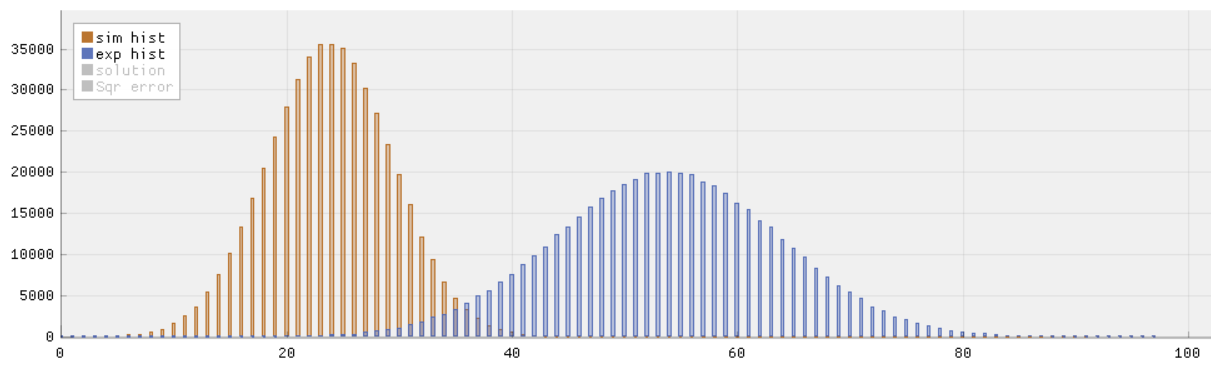
\includegraphics[width=\linewidth]{images/gaus_dist.png}
   \caption{Пример смещенного и сжатого вдвое истинного спектра}
   \label{photo:gaus_dist}
 \end{figure}

Мы генерируем распределение $\tau$ размерности $n$ в соответствии с некоторой идеей лежащего в основе физического процесса и 
выполняем моделирование нашего детектора. Для начала разделим множество значений исходной величины на интервалы 
$(\Delta_{1}, \Delta_{2}, \cdots ,\Delta_{n_{\tau}})$. Дискретным распределением величины будем называть вероятности попадания 
в определенный интервал $p = (p_{1}, p_{2}, \cdots, p_{n_{\tau}})$. Для разбиения множества истинных значений можно использовать 
другие интервалы $(\Delta'_{1}, \Delta'_{2}, \cdots ,\Delta'_{n_{m}})$, но в данной работе будет рассмотрен вариант с одинаковым 
баннингом для измеренных и истинных значений. Количество частиц, по итогам эксперимента детектированных аппаратурой в выделенных 
ячейках, обозначим $m = (m_{1}, m_{2}, \cdots, m_{n_{m}})$ и будем называть измеренным многомерным спектром. 


На этом этапе каждую запись в измеряемом бине (т.е. каждое событие) можно напрямую проследить до ее происхождения. 
Это дает нам хорошо определенную систему линейных отношений между смоделированным истинным и измеренным распределениями: 
$A\tau = m$. Матрица $A$ размера $n_{m} \times n_{\tau}$ строиться следующим образом, 
$A_{ij} = P( \text{ истинное } \in \text{Bin}_{i} \mid \text{зарегистрированное} \in \text{Bin}_{j} )$, 
то есть представляет собой вероятностную матрицу, которая фактически выполняет имитируемую процедуру свертки, обычно она называется матрицей
миграций или матрица откликов.

Например для случая изображенного на рис. \ref{photo:gaus_dist} матрица миграций будет выглядеть следующим образом:

\begin{figure}[h]
   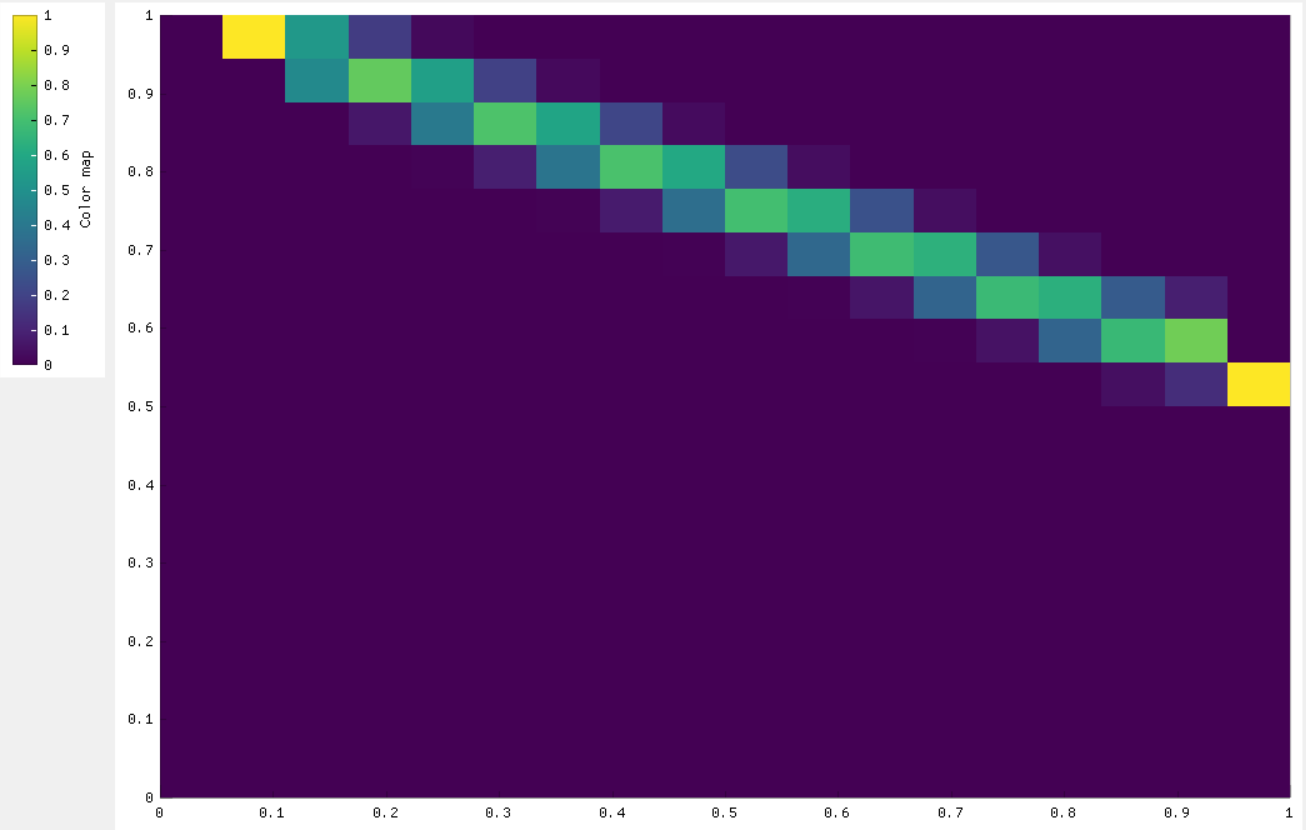
\includegraphics[width=\linewidth]{images/gaus_mig.png}
   \caption{Пример матрицы миграций распределения изображенного на рис. \ref{photo:gaus_dist} }
   \label{photo:gaus_mig}
\end{figure}

Данная матрица является не диагональной, так как, в искажении присутсвует сдвиг. При работе с данными описываюсщие физические частицы, 
матрица миграций чаще всего проходит через главную диагональ.

Непосредственное решение через инверсию матрицы $\tau = A^-1 m$ ,обычно, ведет к неприемлемым результатам, с большой статистической
ошибкой. Хотя сама оценка сосоятельной и несмещенной, но крайне чевствительной к небольшим колебаниям, что продемонстрировано в работе [],
из-за чего не получиться извлеч полезную иформацию из такого из решения задачи таким методом.


\subsection*{Методы обратной свертки}

Существует несколько подходов для уменьшения статистических ошибок, которые являются доработкой прямого метода либо реализуют принципиально
новую идею решения задачи обратной свертки:
\begin{enumerate}
\item SVD-метод основанный на регуляризация Тихонова.
\item Байесовские методы (метод д’Агостини).
\item Метод поправочных коэффициентов.
\end{enumerate}

Далее рассмотрена модификация метода решения предложенного в работе [ ], основанная на методе регулязации сингулярного разложения матриц. 
Данный подход интересен тем, что с его помощью можно использовать особенности, искомого спектра, отражая их в виде дополнительных функций. 
Например, для регулязации Тихонова, используется слагаемое отражающее гладкость распределения, а которое выражается через разность соседних 
линейно занумерованных бинов, для многомерного случая данный подход не работает, так как при переходе из многомерного в одномерный случай 
теряется информация о "многомерном" соседстве, и после не учитывается при решении.

Оценку спектра истинных значений, которая была получена прямым методом, можно представить в виде точки минимума следующей функции: 

\begin{equation}
   \Phi(\tau)=(R\tau-m)^T (R\tau-m) \to min_{\tau}
   \label{min:base}
\end{equation}

Для того чтобы учитывать дополнительно характер распределения, предлагается добавить регулязационное слагаемое или слагаемые, 
которые могут описывать например гладкость. С учетом дополнительного слагаемого система будет иметь следующий вид: 

\begin{equation}
   \Phi(\tau)=(R\tau-m)^T (R\tau-m) + \alpha S(\tau) \to min_{\tau}
   \label{min:svd}
\end{equation}
  
Здесь $S(\tau)$ как раз играет роль регулязатора, а $\alpha$ - это коэффициент сглаживания. Соответственно при $\alpha = 0$ 
получаем исходную систему. При таком подходе могут варьироваться дополнительные слагаемые и методы подбора коэффициентов. 
В данный работе берется за основу метод Картвелишвили и Хокера [ ], который подробно описан в следующей главе. 



\section{Сингулярное разложение матриц}

Сингулярным разложение (или SVD) действительной матрицы $A$ размера $m \times n$ — это ее факторизация вида: 
\begin{equation}
    A = U S V^T 
\end{equation}

где $U$ — ортогональная матрица размера $m \times m$, $V$ — ортогональная матрица размера $n \times n$, а $S$ — диагональная матрица размера 
$m \times n$ с неотрицательными диагональными элементами: 

\begin{equation}
    \begin{array}{l}
        U U^T = U^T U = I, \quad VV ^T = V^T V = I, \\
        S_{ij} = 0 \quad for \ i \neq j, \quad S_{ii} = s_{i} \geq 0
    \end{array}
\end{equation}

Значения на главной диагонали матрицы $S - s_{i}$  называются сингулярными значениями матрицы $A$, а столбцы матриц $U$ и $V$ называются левыми 
и правыми сингулярными векторами. Сингулярные значения содержат очень ценную информацию о свойствах матрицы. Если, например, 
A сама ортогональна, все ее сингулярные значения равны 1. Наоборот, вырожденная матрица будет иметь хотя бы один ноль среди своих 
сингулярных значений. Фактически ранг матрицы — это число ее ненулевых сингулярных значений. Если матрица линейной системы плохо обусловлена, 
а некоторые сингулярные значения матрицы значительно меньше других, система может быть трудной для решения, даже если формально матрица 
имеет полный ранг. Во многих аспектах такие матрицы ведут себя как вырожденные, и SVD предлагает метод решения таких проблем, который 
является общим для малых и нулевых сингулярных значений.

Будем считать, что сингулярные числа $s_{i}$ образуют невозрастающую последовательность, этого легко добиться, поменяв местами пары сингулярных 
значений, одновременно поменяв местами соответствующие столбцы $U$ и $V$. Предположим также, что $m \geq n$, что означает, 
что количество бинов в измеренной гистограмме $m$ не должно быть меньше, чем количество бинов в развернутой гистограмме $\tau$. 
При необходимости можно просто добавить строки нулей в исходную матрицу.




\section[Одномерный случай]{Решение задачи обратной свертки методом \\ регулязации в одномерном случаии}

Для одномерного случая в качестве регулязационного слагаемого предлагаться брать следующую функцию:
\begin{equation}
    S(\tau)= \sum_{i=2}^{n-1} (\tau_{i-1} - 2\tau_{i} + \tau_{i+1})
\end{equation}

отражающую гладкость искомого распределения и является суммой квадратов второй производной по всем интервалам дискретизации. 
Она также может быть записана в матричном виде:
\begin{equation}
    S(\tau) = (C\tau)^T(C\tau)
\end{equation}
где матрица $C$ отражает близость соседних бинов и имеет следующий вид:

\begin{equation}
    C_{m,n} = 
 \begin{pmatrix}
   1 & -1 & 0 & 0 & \cdots & 0 & 0  \\
  -1 &  2 & -1 & 0 & \cdots & 0 & 0  \\
  0 & -1 &  2 & -1 & 0 & \cdots & 0  \\
  \vdots &  & & \ddots & & & \vdots \\
  0  & 0  & 0 & 0 & \cdots & -1 & 1
 \end{pmatrix}
\end{equation}

Следующая задачи минимизации

\begin{equation}
 \Phi(\tau)=(R\tau-m)^T (R\tau-m) + \alpha(C\tau)^T(C\tau) \to min_{\tau}
\end{equation}

\begin{equation}
    \begin{bmatrix}
        RC^-1 \\
        \sqrt{a} \cdot I
    \end{bmatrix}
    C\tau = 
    \begin{bmatrix}
        m \\
        0
    \end{bmatrix}
\end{equation}


Алгоритм общий решения задачи:

\begin{enumerate}
    \item Выполняем сингулярное разложение матрицы A \\
    $USV^T \tau = m.$

    \item Делаем замену $z = V^T\tau$. Получаем $USz = m.$

    \item $U$ - ортогональная, это значит что обратная матрица ровна транспонированной. Домножая систему на $U^{-1}$ получаем $Sz=U^Tm$.

    \item Далее делаем замену $d=U^Tm$, и система принимает вид $Sz=d$.

    \item Отсюда находим $z_{i} = d_{i} / s_{i}$, В матрице сингулярных значений, элементы находятся только на главной диагонали, 
    поэтому рассматриваем просто вектор $s$.

    \item Решение системы находим находим следующим образом $\tau = Vz$.
\end{enumerate}

При решение переопределенной системы, отличия будут при вычислении вектора $z$, теперь его значения будут вычисляться как:
$z_{i} = \frac{d_{i}}{s_{i}} \cdot \frac{s^2_{i}}{s^2_{i} + \alpha}$ (при $\alpha = 0$ решение системы
совпадает с решением \refeq{min:base}).

Данный алгоритм не зависит от регулязационного слагаемого и может использоваться любого другого со схожей идеей. 
Например в качестве функции регуляризации можно выбрать сумму квадратов оценок, других порядков или использовать формулы численного 
дифференцирования с более высоким уровнем погрешности.




\section[Многомерный случай]{Решение задачи обратной свертки методом \\ регулязации в многомерном случаии}

\begin{equation}
 k_{ij} =
  \begin{cases}
    deg(\Delta_{i}) & \quad \text{ при } i = j \\
    -1              & \quad i \neq j  \text{ , и } \Delta_{i} \Delta_{j} \text{- соседи } \\
    0               & \quad \Delta_{i} \Delta_{j} \text{ - не являются соседними }
  \end{cases}
\end{equation}


\begin{equation}
 k_{ij} =
  \begin{cases}
    \displaystyle\sum_{k\neq i} w(\Delta_{i}, \Delta_{k}), \text{ при } \ i = j \\
    -w( \Delta_{i}, \Delta_{j} ), \text{ при } i \neq j
  \end{cases}
\end{equation}





\chapter{Псевдокод}

Пакет \href{https://www.ctan.org/pkg/algorithm2e}{algorithm2e}
предлагает широкий спектр инструментов для создания и оформления псевдокода.
Также имеется возможность делать ссылки на строки кода.
Например, в строке~\ref{alg:lDoWhile} алгоритма~\ref{alg:quicksort}
целиком содержится цикл типа \texttt{do-while}.

\SetAlgorithmName{Алгоритм}{Список алгоритмов}{} % Название на русском
\SetAlgoCaptionSeparator{.} % Отделяем название алгоритма от его номера точкой
%\SetAlgoLined % Вертикальные линии, соединяющие начало и конец блока
\DontPrintSemicolon % Не печатать точку с запятой
\SetKwProg{Proc}{Procedure}{}{end} % Команда для процедуры
\SetKwProg{Fn}{Function}{}{end} % Команда для функции
% Описание входных и выходных данных
\SetKwInOut{Input}{Вход}
\SetKwInOut{Output}{Выход}
\SetKwRepeat{DoWhile}{do}{while} % Создаем цикл do-while
\SetKwBlock{Loop}{loop}{endloop} % Безусловный цикл
\begin{algorithm}
	\caption{Быстрая сортировка} % Заголовок
	\label{alg:quicksort}
	% Обозначения ключевых (входных-выходных) данных алгоритма
	\SetKwArray{Array}{A} % Массив
	\SetKwData{Low}{b}
	\SetKwData{High}{e}
	% Названия новых процедур и функций
	\SetKwFunction{QuickSort}{QuickSort}
	\SetKwFunction{Partition}{Partition}
	% Описание входа-выхода
	\Input{ массив \Array, индексы начала \Low и конца \High сортируемого фрагмента}
	\Output{ массив \Array, отсортированный по возрастанию}
	\BlankLine
	% Непосредственно процедура QuickSort
	\Proc{\QuickSort{\Array, \Low, \High}}{
		\If{$\Low < \High$}{
			$m \leftarrow$ \Partition{\Array, \Low, \High}\;
			\QuickSort{\Array, \Low, $m$}\;
			\QuickSort{\Array, $m+1$, \High}\;
		}
	}
	\BlankLine
	% Функция Partition
	\Fn{\Partition{\Array, \Low, \High}}{
		$v \leftarrow$ \Array{\Low}\;
		$i \gets \Low - 1$\;
		$j \gets \High + 1$\;
		\Loop{
			\DoWhile{$\Array{$i$} < v$}{
				$i \gets i + 1$\;
			}
			\lDoWhile{$\Array{$j$} > v$}{$j \gets j - 1$} \label{alg:lDoWhile}
			\If{$i \ge j$}{\Return{$j$}\;}
			поменять местами \Array{$i$} и \Array{$j$}\;
		}
	}
\end{algorithm}


\chapternonum{Заключение}

% В заключении подводятся итоги выполненной работы, рассказывается о~том, что удалось и~что не~удалось сделать, описываются перспективы продолжения исследований.
\renewcommand\bibname{Список литературы}
\bibliographystyle{ugost2003}
\bibliography{bibliography}

% Приложения
\appendix
	
% Настраиваем общее для всех языков оформление листинга
\lstset{
	%	breaklines=true,
	%	frame=l,
	%	showstringspaces=false,
	tabsize=4, % длина табуляции в пробелах
	formfeed=\newpage, % реакция на символ "form feed"
	extendedchars=true, % используем неанглийские буквы
	basicstyle=\ttfamily, % базовый стиль
%	keywordstyle=\bfseries, % стиль ключевых слов (попробуйте \pmb если \bfseries не работает)
	commentstyle=\rmfamily\itshape, % стиль для комментариев
	stringstyle=\slshape, % стиль строк в кавычках
	numbers=left, % где проставляем номера строк; возможные значения: none, left, right
	numbersep=1em, % расстояние (по горизонтали) от номеров строк до кода
	stepnumber=1, % шаг отображения номеров строк. Если 1, то каждая строка помечается номером
	numberstyle=\footnotesize\color{black}, % стиль для номеров строк
}


% \chapter{Исходный код программы на C++}
% \label{app:source}

% Настраиваем оформление листинга для C++
% \lstdefinestyle{cpp}{
% 	language=[ANSI]C++,
% 	morekeywords={string, list} % расширяем список ключевых слов
% }

% Загружаем код из файла
% \lstinputlisting[style=cpp]{sort.cpp} 

% Части вашего текста можно хранить в отдельных файлах (это особенно удобно для приложений) и включать их в основной файл с помощью команды \input{имя файла}
% % !TeX encoding = windows-1251
% !TEX root = diplExample.tex

\chapter{Исходный код программы на Python}
\label{app:Python}

% Настраиваем оформление листинга для Python
\lstdefinestyle{Python}{
	language=Python,
	morekeywords={models, lambda, forms, self} % расширяем список ключевых слов
}

% Определяем ограничители для ввода меток на строки кода
% Для этого используем редкие для языка комбинации символов
\lstset{escapeinside={|@}{@|}}

Пример кода на Python 3 (взят с \href{http://python3.codes/alan-turings-automatic-machine/}{официального сайта}), реализующий симулятор машины Тьюринга для сложения унарных чисел (типа $11 + 111$).
Листинг позволяет делать (автоматическую) ссылку на какую"=нибудь строку. Например, на строку~\ref{lst:1} с командой \texttt{print(tape)}.

% Листинг кода на Python
%# Turing Machine simulator to add unary numbers (e.g. 11 + 111)
%#
\begin{lstlisting}[style=Python]
# prog is indexed by the current tape symbol (0 or 1) 
# and then by state (a kind of instruction pointer) 
# to get an 'instruction' comprising:
#   symbol to write on current tape position,
#   head action (-1 = move left, +1 = move right)
#   next state (like a goto jump).

#       symbol 0    symbol 1
prog = [[(1, +1, 1), (1, +1, 0)],         # state 0
		[(0, -1, 2), (1, +1, 1)],         # state 1
		[(0, +1, 2), (0, +1, 9)]]         # state 2
tape = [1,1,0,1,1,1,0,0,0]                # The data tape
head = 0                                  # head position on tape
state = 0                                 # instruction pointer
print(tape)  |@\label{lst:1}@|
while state != 9:                         # while not halt:
	symbol = tape[head]                   # read current tape symbol
	symbol, dir, state = t = prog[state][symbol] # lookup instruction
	print(' ' * (head * 3 + 1)+ '^  ' + str(t)) # display progress
	tape[head] = symbol                   # write new symbol on tape
	print(tape)
	head = head + dir                           # move tape head
\end{lstlisting}



% Конец документа
\end{document}
